\documentclass[
	25pt,
	a0paper, 
	portrait,
	blockverticalspace=-3em,
	margin=.5in,
	innermargin=0mm
]{tikzposter}

\tikzposterlatexaffectionproofoff

\usepackage{blindtext}
\usepackage{comment}
\usepackage{lipsum}
\usepackage{wrapfig}
\usepackage[sort&compress, numbers]{natbib}
\usepackage{bibentry}
\usepackage{lipsum}
\usepackage{bm}
\usepackage{booktabs}
\usepackage{xtab}
\usepackage{caption}
\usepackage{easy-todo}
%\usepackage{hyphenat}


\graphicspath{{figures}{figures/graphics}}
\bibliographystyle{abbrvnat}

\renewcommand{\bibsection}{}

	% Theme

%%%%%% UVM COLORS
\definecolor{uvm-green}{RGB}{ 0, 113, 86}
\definecolor{bright-green}{RGB}{103, 172, 71}
\definecolor{sky-blue}{RGB}{167,212,238}

\definecolor{bright-yellow}{RGB}{255,212,22}
\definecolor{mid-blue}{RGB}{141,212,238}
%%%%%%



%%%%% Theme
\usetheme{Simple}
\colorlet{titlebgcolor}{uvm-green}
\colorlet{blocktitlefgcolor}{bright-green}
\colorlet{notebgcolor}{sky-blue}
%%%



% Title
%%%%% Title block
\title{
	\parbox{\titlewidth}{
		\centering
			Smoking Reduction Trajectories and their Association with Smoking Cessation
			\vspace{.5em}
		}
	}

%\title{Smoking Reduction Trajectories and their Association with Smoking Cessation}
%\title{text}

\author{\large Anthony Barrows$^{1,2}$, Elias Klemperer$^{1,3}$, Hugh Garavan$^{1}$, Nicholas Allgaier$^{1,2}$, Nicola Lindson$^4$, Gemma Taylor$^5$}
%\date{\today}
\institute{
	$^1$ 
\includegraphics[width=3.25in]{UVMLogoOutlineWhite}
	$^2$ 
\includegraphics[width=1in]{complexsystems}
	$^3$ 
\includegraphics[width=2in]{vcbh}
	$^4$ 
\includegraphics[width=2in]{oxford_logo}
	$^5$ 
\includegraphics[width=1.5in]{bath_logo}
}
%%%%%%%%%



\makeatletter
\def\title#1{\gdef\@title{\scalebox{\TP@titletextscale}{%
			\begin{minipage}[t]{\linewidth}
				\centering
				#1
				\par
			\end{minipage}
}}}
\makeatother


\makeatletter
\newcommand\insertlogoi[2][]{\def\@insertlogoi{\includegraphics[#1]{#2}}}
\newcommand\insertlogoii[2][]{\def\@insertlogoii{\includegraphics[#1]{#2}}}
\newlength\LogoSep
\setlength\LogoSep{0pt}
%
%\insertlogoi[width=8cm]{example-image-a}
%\insertlogoii[width=8cm]{example-image-b}
%
%\insertlogoi[width=8cm]{example-image-a}
%\insertlogoii[width=8cm]{example-image-b}

\renewcommand\maketitle[1][]{  % #1 keys
	\normalsize
%	\small
	\setkeys{title}{#1}
	% Title dummy to get title height
	\node[transparent,inner sep=\TP@titleinnersep, line width=\TP@titlelinewidth, anchor=north, minimum width=\TP@visibletextwidth-2\TP@titleinnersep]
	(TP@title) at ($(0, 0.5\textheight-\TP@titletotopverticalspace)$) {\parbox{\TP@titlewidth-2\TP@titleinnersep}{\TP@maketitle}};
	\draw let \p1 = ($(TP@title.north)-(TP@title.south)$) in node {
		\setlength{\TP@titleheight}{\y1}
		\setlength{\titleheight}{\y1}
		\global\TP@titleheight=\TP@titleheight
		\global\titleheight=\titleheight
	};
	
	% Compute title position
	\setlength{\titleposleft}{-0.5\titlewidth}
	\setlength{\titleposright}{\titleposleft+\titlewidth}
	\setlength{\titlepostop}{0.5\textheight-\TP@titletotopverticalspace}
	\setlength{\titleposbottom}{\titlepostop-\titleheight}
	
	% Title style (background)
	\TP@titlestyle
	
	% Title node
	\node[inner sep=\TP@titleinnersep, line width=\TP@titlelinewidth, anchor=north, minimum width=\TP@visibletextwidth-2\TP@titleinnersep]
	at (0,0.5\textheight-\TP@titletotopverticalspace)
	(title)
	{\parbox{\TP@titlewidth-2\TP@titleinnersep}{\TP@maketitle}};
	
%	\node[inner sep=0pt,anchor=west] 
%	at ([xshift=-\LogoSep]title.west)
%	{\@insertlogoi};
%	
%	\node[inner sep=0pt,anchor=east] 
%	at ([xshift=\LogoSep]title.east)
%	{\@insertlogoii};
	
	% Settings for blocks
	\normalsize
	\setlength{\TP@blocktop}{\titleposbottom-\TP@titletoblockverticalspace}
}
\makeatother


\begin{document}
	\maketitle[titletoblockverticalspace=0em]
%		\maketitle 
\block{Introduction}
	{
	\centering
		\begin{columns}
			\column{0.45}
			\begin{minipage}[]{0.525\linewidth}
				\begin{itemize}
					\large
					\item Smoking is the leading cause of premature death and preventable illness worldwide \citep{worldhealthorganizationWHOReportGlobal2011}.
					\item A prior Cochrane review found that reduction interventions are no more or less effective than quitting abruptly \citep{lindsonSmokingReductionInterventions2019}.
						\item However, little is known about how people reduce their smoking and which smoking reduction patterns predict better cessation outcomes.
				\end{itemize}
		    \end{minipage}
			\column{0.45}
				\fbox{\begin{minipage}[]{0.45\linewidth}
						\vspace{1em}
						\begin{itemize}
							\large \raggedright
							\item When people are asked to reduce smoking, how do people choose to do so? 
							\item Are there smoking or demographics associated with certain reduction patterns?
							\item Which patterns of reduction are associated with better cessation outcomes?
						\end{itemize}
					\vspace{1em}
				\end{minipage}}
		\end{columns}
	}
		
\block{Methods}
	{

		\begin{columns}
			\column{0.3}
				\begin{minipage}[]{0.31\linewidth}
					\large
					\section*{Data}
	
					\begin{itemize}
						\raggedright
						\item Smoking and demographic information from 5 clinical trials of NRT	\cite{wennikeSmokingReductionPromotes2003,rennardEfficacyNicotineInhaler2006,bolligerSmokingReductionOral2000,batraSmokingReductionTreatment2005,hausteinDoubleblindRandomizedPlacebocontrolled2001}					
						\item Baseline and follow-up (weeks 2, 10, 18, and 26) CPD were recorded
						\item CPD and expired breath carbon monoxide (CO) collected at week 56
						\item Anxiety and depression (from SCQoL\cite{OlufadeEtAl1999}), and nicotine dependence (FTND\cite{fagerstromNicotineAddictionIts1990}) were recorded at baseline
						\item Participants in the included trials were:
							\begin{itemize}
									\item enrolled if they smoked $\geq 15$ CPD, made a recent quit attempt, were currently unmotivated to quit, and wanted to reduce their smoking.
									\item randomly assigned to receive active or placebo NRT (gum or inhaler)
%									gum ($n=1053$, 59.1\%) or inhaler ($n=730$, 40.9\%).
									\item told to reduce their smoking as much as possible.
								\end{itemize}
					\end{itemize}
				\end{minipage}
			\column{0.4}
				\begin{minipage}[]{0.375\linewidth}
				
				\begin{tikzfigure}
					\captionof{table}{Baseline demographic, smoking, and behavioral characteristics.}
					\begin{tabular}{lllll}
						\toprule
						& Overall & Class 1       & Class 2       & Class 3       \\
						\cmidrule{2-5}
						N (\%)                         & 1783 (100)      & 186 (10.4)    & 803 (45.0)    & 794 (44.5)    \\
						\midrule
						Study Site (\%)                &                 &               &               &               \\
						\hspace{3mm}Australia                      & 360 (20.2)      & 32 (17.2)     & 159 (19.8)    & 169 (21.3)    \\
						\hspace{3mm}Denmark                        & 340 (19.1)      & 35 (18.8)     & 175 (21.8)    & 130 (16.4)    \\
						\hspace{3mm}Germany                        & 353 (19.8)      & 60 (32.3)     & 153 (19.1)    & 140 (17.6)    \\
						\hspace{3mm}Switzerland                    & 301 (16.9)      & 29 (15.6)     & 139 (17.3)    & 133 (16.8)    \\
						\hspace{3mm}USA                            & 429 (24.1)      & 30 (16.1)     & 177 (22.0)    & 222 (28.0)    \\
						Active NRT (\%) & 900 (50.5)      & 125 (67.2)    & 413 (51.4)    & 362 (45.6)    \\
						Sex = Male (\%)                & 798 (44.8)      & 96 (51.6)     & 357 (44.5)    & 345 (43.5)    \\
						Age (m(sd))                & 44.10(10.72)    & 45.79 (11.41) & 44.26 (10.52) & 43.53 (10.73) \\
						FTND (m(sd))      & 6.14 (2.00)     & 5.60 (2.13)   & 6.11 (2.01)   & 6.30 (1.94)   \\
						CPD (m(sd))       & 27.32 (9.73)    & 25.65 (10.37) & 27.42 (9.78)  & 27.62 (9.50)  \\
						SCQoL Anxiety (m(sd))              & 0.45 (0.85)     & 0.41 (0.83)   & 0.41 (0.82)   & 0.51 (0.90)   \\
						SCQoL Depression (m(sd))       & 0.29 (0.69)     & 0.29 (0.69)   & 0.26 (0.67)   & 0.32 (0.71) \\
						\bottomrule
					\end{tabular}
				\label{tab:demographics}
	
				\end{tikzfigure}
				
				
				\end{minipage}
			\column{0.3}
				\begin{minipage}[]{0.29\linewidth}
					\large
					\section*{Analysis}
					\begin{enumerate}
						\raggedright
						\item We estimated smoking trajectories using latent class analysis (LCA) as a function of percent reduction in CPD.  Participants were assigned to the most likely latent class.
						
						\item We used regularized regression (i.e., elastic net) under a nested cross validation scheme to predict latent class using baseline and demographic characteristics (see Table \ref{tab:demographics}).
						
						\item We predicted biochemically-verified smoking status (CO < 6ppm) at week 52 using baseline and demographic characteristics, plus latent class.
						
					\end{enumerate}
								\vspace{1em}
				
					\fbox{\begin{minipage}{\linewidth}
						\small
						\begin{itemize}
							\item Pre-registered protocol: \texttt{https://osf.io/qh378/}
							\item Analytical code: \texttt{https://github.com/ajbarrows/mcneil-lca}
						\end{itemize}
				\end{minipage}}
				


			\end{minipage}
	\end{columns}

		}
	

\block{Results}
	{
	\centering
	\begin{columns}
		\column{0.4}
		\begin{minipage}[]{0.45\linewidth}
			\large
			\subsection*{Participants}
			\begin{itemize}
				\item 108/2066 participants were excluded for missing values. 
				\item  Resulting $n=1783$:
				\begin{itemize}
					\item From five countries
					\item 44.8\% male, mean age 44.10 $\pm$ 10.72 years
					\item Smoked an average of 27.32 $\pm$ 9.73 CPD
				\end{itemize}
			\end{itemize}
			\subsection*{Latent Class Analysis}

			\begin{itemize}
				\item Class 1: 10.43\% initially reduced and nearly eliminated smoking
				\item Class 2: 45.04\% reduced by nearly 50\% and remained
				\item Class 3: 44.53\% initially reduced but reverted to their baseline smoking
			\end{itemize}
		
			\subsection*{Predicting Latent Class}
			\begin{itemize}
				\item Demographic data and baseline characteristics (e.g., smoking and quit behavior, FTND, SF-36, trial treatment group) were used as independent variables
%				\item After column-wise ($>25\%$ values missing) and list-wise ($\geq 7$ variables missing) deletion, remaining missing data was imputed within age/sex/study site groups
				\item Latent class was used as the dependent variable
				\item One cross-validated elastic net logistic regression for each latent class (i.e., one-versus-all)
				\item All models performed better than chance:
				\begin{itemize}
					\item Class 1 test AUC = 0.766, $p<.001$. Tended to be older with lower anxiety and nicotine dependence, more likely to have received active NRT.
					\item Class 2 test AUC = 0.569, $p=.008$ No clear pattern of characteristics.
					\item Class 3 test AUC = 0.523, $p<.001$ Inverse of class one: higher nicotine dependence, more likely to have received placebo NRT.
				\end{itemize}
			\end{itemize}
					\innerblock{Conclusions}{%
			\begin{itemize}
				\large 
				\item \textbf{Examining latent trajectories in smoking behavior among people not motivated to quit revealed three distinct patterns}
				\item \textbf{One of these trajectories was nearly twice as likely as the others to achieve cessation}
				\item \textbf{Smoking reduction in the first two weeks after intervention by $\bm{\geq 50\% \rightarrow}$ substantially increased cessation likelihood}
			\end{itemize}
		}
		\end{minipage}
		\column{0.5}
%		\vspace{-8mm}
		\begin{minipage}[]{0.5\linewidth}
				\begin{tikzfigure}[]
						\centering
						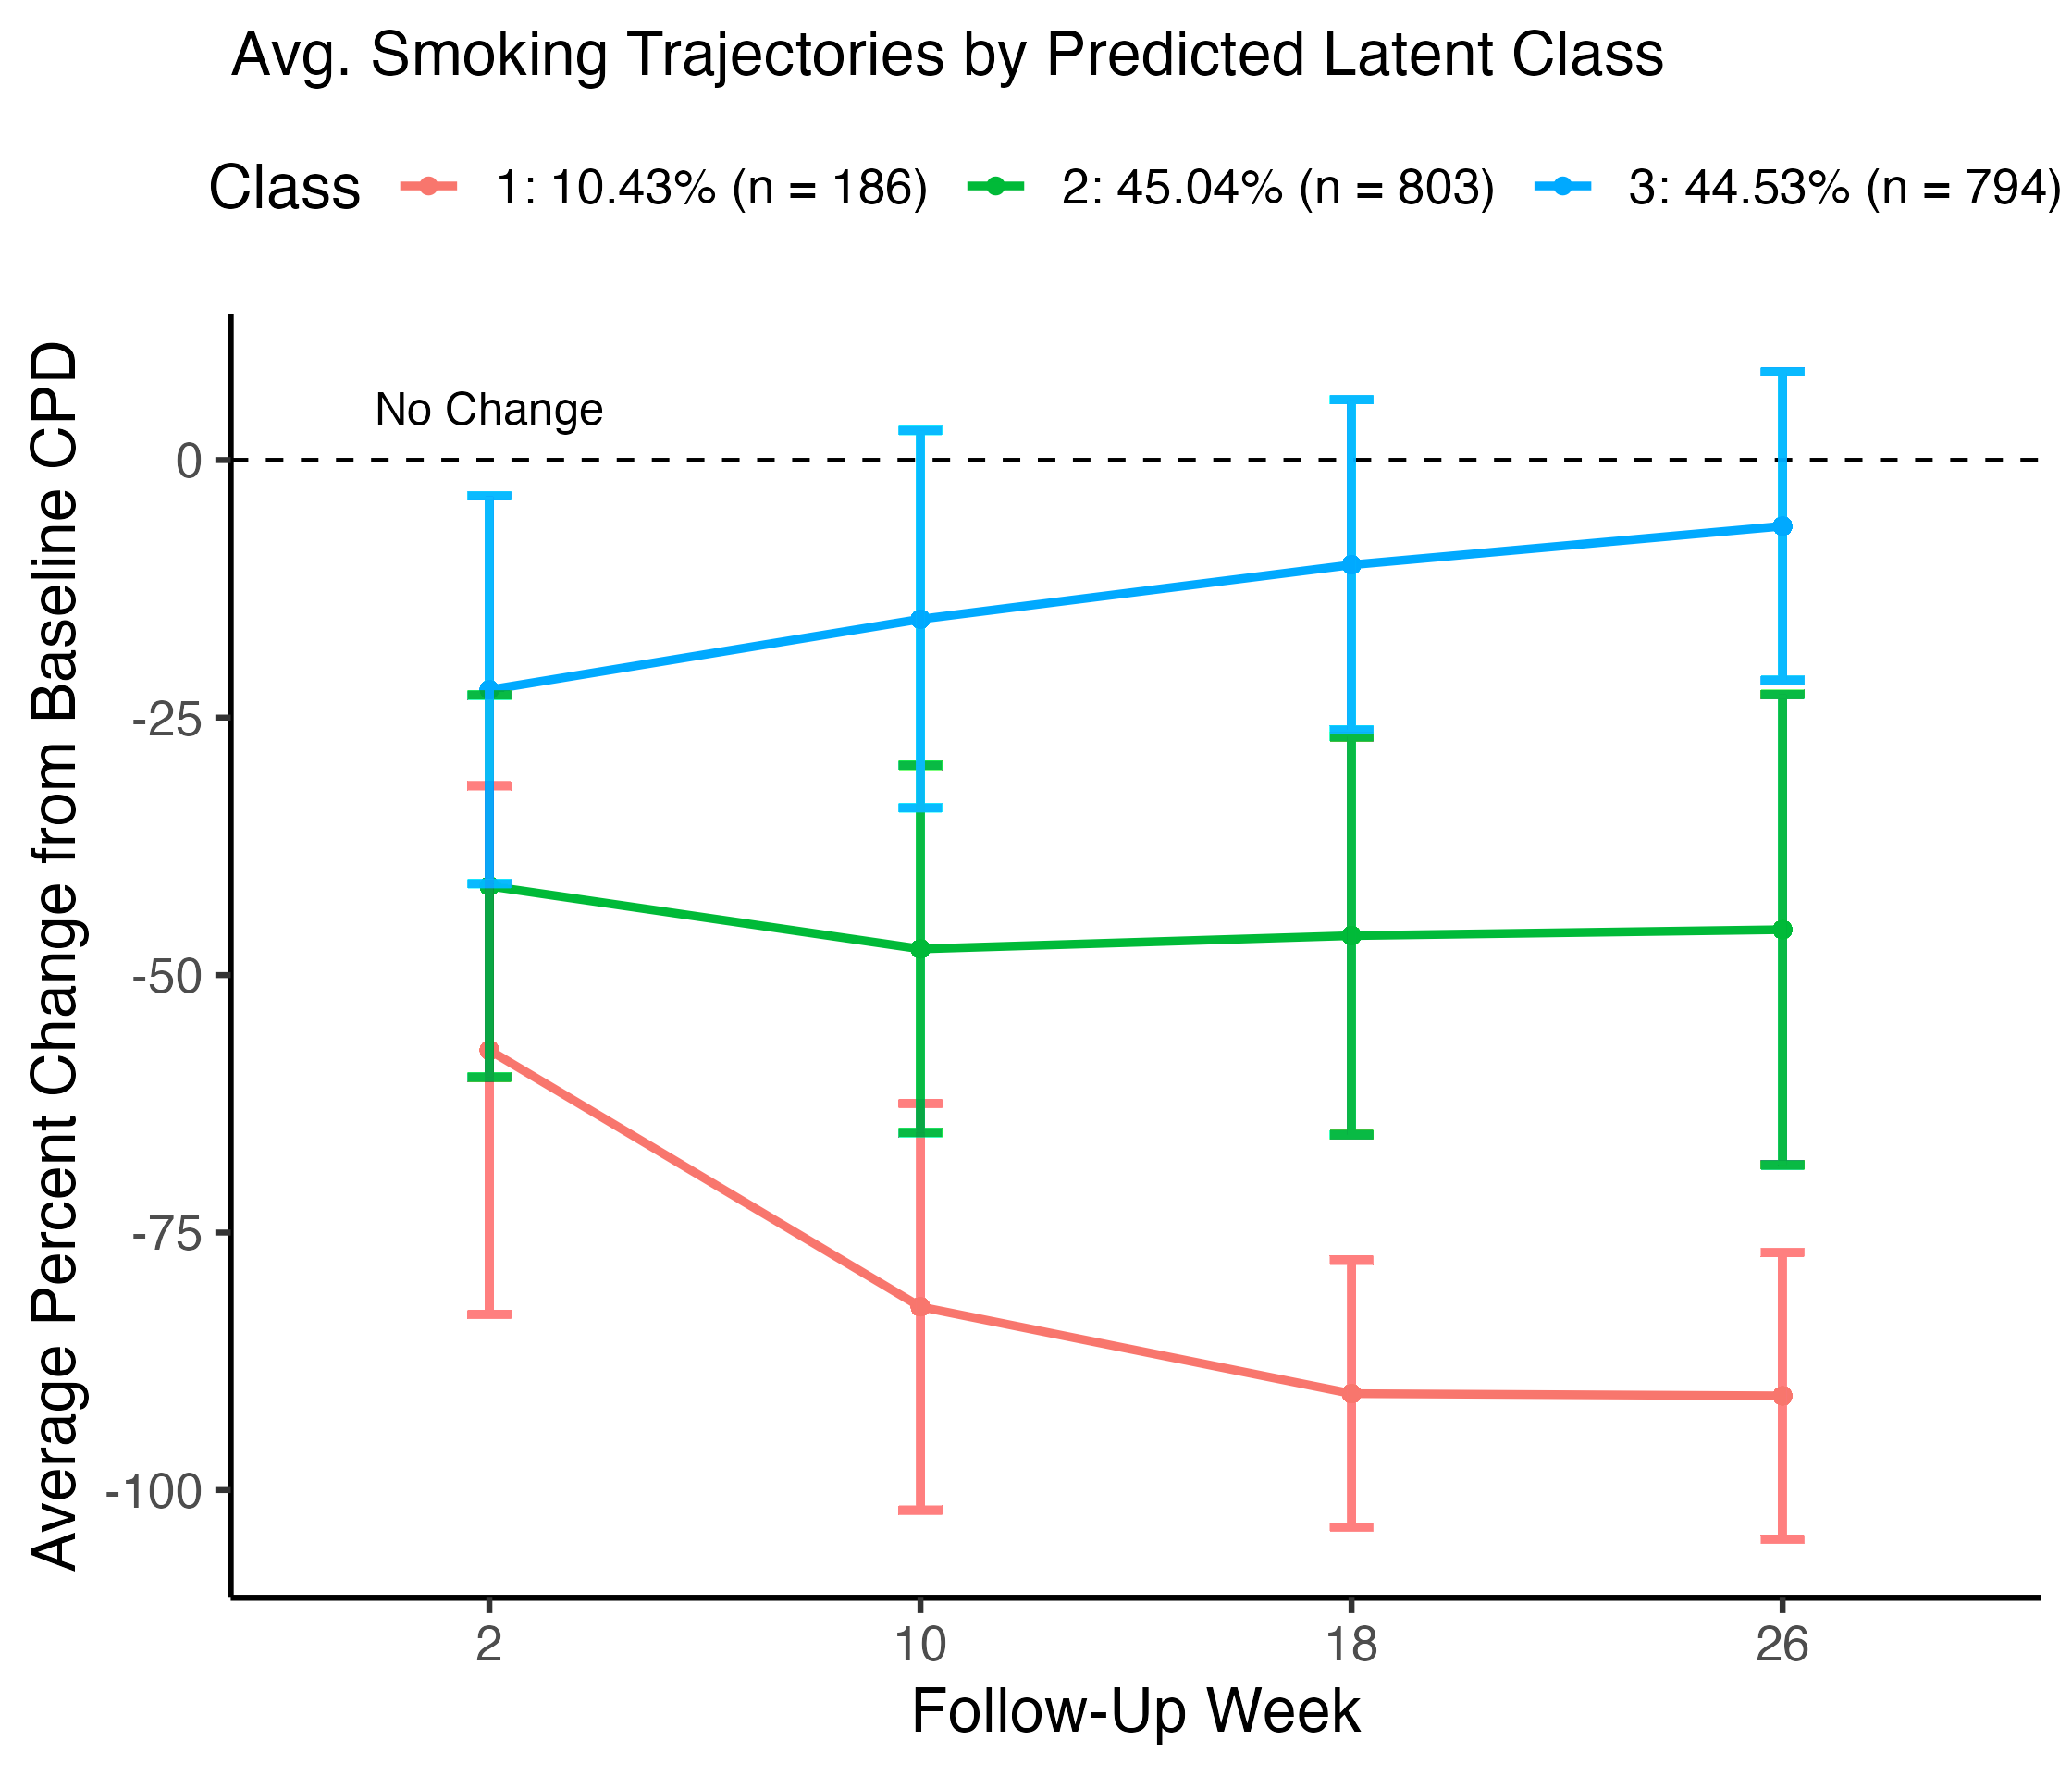
\includegraphics[width=.9\linewidth]{smoking_traj}
					\end{tikzfigure}
					\subsection*{Predicting Smoking Status }
						\large
						\begin{itemize}
							\raggedright
								\item 122/1783 (6.8\%) achieved biochemically-verifiable smoking cessation at week 52:
								\begin{itemize}
										\item Class 1: 70/186 (37.6\%); Class 2: 34/803 (4.2\%); Class 3: 18/776 (2.3\%)
									\end{itemize}
								\item Elastic net logistic regression predicting smoking cessation using
								\begin{itemize}
										\item baseline characteristics alone: AUC = $0.632 \pm 0.006$, $p<.001$
										\item baseline characteristics plus latent class: AUC = $0.776 \pm 0.010$, $p<.001$
									\end{itemize}
								\item \textbf{Adding latent class as an independent variable improved cessation prediction by 14.4\%}
							\end{itemize}
						\centering
						\vspace{1mm}
					\fbox{e-mail \texttt{Anthony.Barrows@uvm.edu}}
			\end{minipage}
%			\begin{minipage}{0.5\linewidth}
%				\bibliography{bibliography}
%			\end{minipage}
%		\begin{minipage}{0.45\linewidth}
%					\block{References}{%
%				%			\footnotesize
%				%			\bibliography{bibliography}
%				test
%			}
%		\end{minipage}

		
	\end{columns}

}

\begin{columns}
	\column{0.5}
	\block{}{%
		\begin{minipage}[]{\linewidth}
			\raggedright \small
			This work is supported by
				\begin{itemize}
						\item NIH (NIDA T32DA045593 and NIGMS P20GM103644)
						\item Cancer Research UK (PRCPJT-Nov22/100012, PPRCPJT\textbackslash100,023, and C56067/A21330)
						\item The University of Oxford and  NHS Greater Manchester Integrated Care
				\end{itemize}
				\hrule
				\vspace{1mm}
		\end{minipage}

		\begin{minipage}[]{\linewidth}
			\begin{tikzfigure}
				\begin{tabular}{l|l|l|l}
					
					& \begin{minipage}{0.1\columnwidth}
						\small \raggedright
						Tobacco Industry
					\end{minipage} & 
					\begin{minipage}{0.2\columnwidth}
						\small
						\raggedright E-cigarette \& nicotine product industry 
					\end{minipage} &
					\begin{minipage}{0.1\columnwidth}
						\small \raggedright
						Pharma Industry 
					\end{minipage} \\
					\begin{minipage}{0.5\columnwidth}
						\small
						The work being presented has received funding or other means of support from any of the following sources:
						\vspace{2mm}
					\end{minipage} & No & No & No\\
					\midrule
					
					\begin{minipage}{0.5\columnwidth}
						\small
						Any of the authors have received funding (including consultancy) from any of the following sources in the past 5 years:
					\end{minipage} &No &No &No
					
				\end{tabular}
			\end{tikzfigure}
		\end{minipage}
}

	
	\column{0.5}
	\block{}{%
	\begin{minipage}[]{\linewidth}
		\subsection*{References}
			\tiny
			\bibliography{bibliography}
		\end{minipage}	
}
\end{columns}

%\block{Acknowledgements}{}

%		\innerblock{Conclusions}{%
	%			\begin{itemize}
		%				\normalsize
		%				\item Examining latent trajectories in smoking behavior among people not motivated to quit revealed three distinct patterns
		%				\item One of these trajectories was nearly twice as likely as the others to achieve cessation
		%				\item Smoking reduction in the first two weeks after intervention by $\bm{\geq 50\% \rightarrow}$ substantially increased cessation likelihood
		%			\end{itemize}
	%		}
%		\small \centering \normalcolor
%		\vspace{1mm}
%		\fbox{e-mail \texttt{Anthony.Barrows@uvm.edu}}
%
%\block{}{%
%	\begin{columns}
%		\column{0.45}
%			\begin{minipage}[]{\linewidth}
%					\raggedright \small
%					This work is supported by
%					\begin{itemize}
%							\item NIH (NIDA T32DA045593 and NIGMS P20GM103644)
%							\item Cancer Research UK (PRCPJT-Nov22/100012, PPRCPJT\textbackslash100,023, and C56067/A21330)
%							\item The University of Oxford and  NHS Greater Manchester Integrated Care
%						\end{itemize}
%				\end{minipage}
%%						\begin{minipage}{0.45\linewidth}
%%				\small
%%				\bibliography{bibliography}
%%			\end{minipage}
%			\begin{minipage}[]{0.45\linewidth}
%					\begin{tikzfigure}
%							\begin{tabular}{l|l|l|l}
%									
%									& \begin{minipage}{0.1\columnwidth}
%											\small \raggedright
%											Tobacco Industry
%										\end{minipage} & 
%									\begin{minipage}{0.2\columnwidth}
%											\small
%											\raggedright E-cigarette \& nicotine product industry 
%										\end{minipage} &
%									\begin{minipage}{0.1\columnwidth}
%											\small \raggedright
%											Pharma Industry 
%										\end{minipage} \\
%									\begin{minipage}{0.45\columnwidth}
%											\small
%											The work being presented has received funding or other means of support from any of the following sources:
%											\vspace{2mm}
%										\end{minipage} & &&\\
%									\midrule
%									
%									\begin{minipage}{0.45\columnwidth}
%											\small
%											Any of the authors have received funding (including consultancy) from any of the following sources in the past 5 years:
%										\end{minipage} &&&
%									
%								\end{tabular}
%						\end{tikzfigure}
%				\end{minipage}
%			\column{0.45}
%						\begin{minipage}[t]{0.5\linewidth}
%				\tiny
%				\bibliography{bibliography}
%			\end{minipage}
%
%
%	\end{columns}
%}



%\block{}{%
	%	\vspace{-20mm}
	%	\begin{minipage}[]{\linewidth}
		%		\raggedright \small
		%		This work is supported by
		%		
		%		\begin{itemize}
			%			\small
			%			
			%			\item NIH (NIDA T32DA045593 and NIGMS P20GM103644)
			%			\item Cancer Research UK (PRCPJT-Nov22/100012, PPRCPJT\textbackslash100,023, and C56067/A21330)
			%			\item The University of Oxford and  NHS Greater Manchester Integrated Care
			%		\end{itemize}
		%		
		%		%
		%		%	\bibliography{bibliography}
		%		
		%	\end{minipage}
	%	\hrule
	%	\begin{minipage}[]{\linewidth}
		%		
		%		\begin{tikzfigure}
			%			\begin{tabular}{l|l|l|l}
				%				
				%				& \begin{minipage}{0.1\columnwidth}
					%					\small \raggedright
					%					Tobacco Industry
					%				\end{minipage} & 
				%				\begin{minipage}{0.2\columnwidth}
					%					\small
					%					\raggedright E-cigarette \& nicotine product industry 
					%				\end{minipage} &
				%				\begin{minipage}{0.1\columnwidth}
					%					\small \raggedright
					%					Pharma Industry 
					%				\end{minipage} \\
				%				\begin{minipage}{0.5\columnwidth}
					%					\small
					%					The work being presented has received funding or other means of support from any of the following sources:
					%					\vspace{2mm}
					%				\end{minipage} & &&\\
				%				\midrule
				%				
				%				\begin{minipage}{0.5\columnwidth}
					%					\small
					%					Any of the authors have received funding (including consultancy) from any of the following sources in the past 5 years:
					%				\end{minipage} &&&
				%				
				%			\end{tabular}
			%		\end{tikzfigure}
		%	\end{minipage}
	%}






%	\tiny
%	\bibliography{bibliography}
%\block[]

%\block{}{%
	%	\fbox{%
		%			e-mail \texttt{Anthony.Barrows@uvm.edu}
		%	}
	%}

%
%\begin{columns}
%	\column{0.5}
%
%
%
%\column{0.5}

	
%	\begin{tikzfigure}
%		\begin{tabular}{l|l|l|l}
%		
%			& \begin{minipage}{0.05\columnwidth}
%			\small
%				Tobacco Industry
%			\end{minipage} & 
%			\begin{minipage}{0.125\columnwidth}
%				\small
%					\raggedright E-cigarette \& nicotine product industry 
%			\end{minipage} &
%			\begin{minipage}{0.05\columnwidth}
%				\small
%				Pharma Industry 
%			\end{minipage} \\
%			\begin{minipage}{0.15\columnwidth}
%				\small
%				The work being presented has received funding or other means of support from any of the following sources:
%				\vspace{2mm}
%			\end{minipage} & &&\\
%		\midrule
%
%		\begin{minipage}{0.15\columnwidth}
%			\small
%						Any of the authors have received funding (including consultancy) from any of the following sources in the past 5 years:
%		\end{minipage} &&&
%
%		\end{tabular}
%	\end{tikzfigure}
	
%
%	\block[]{}{
%
%}

%\end{columns}


%
%
%
%
%\block{}{
%\begin{columns}
%	\centering
%	\column{0.5}
%	\block{}
%	{\vspace{14em}
%		\fbox{e-mail \texttt{Anthony.Barrows@uvm.edu}}
%	}
%	\column{0.5}
%	\begin{minipage}[c]{0.5\linewidth}
%		\block{Acknowledgements}{
%			This work is supported by
%			
%			\begin{itemize}
%				
%				\item NIH (NIDA T32DA045593 and NIGMS P20GM103644)
%				\item Cancer Research UK (PRCPJT-Nov22/100012, PPRCPJT\textbackslash100,023, and C56067/A21330)
%				\item The University of Oxford and  NHS Greater Manchester Integrated Care
%			\end{itemize}
%			
%			%
%			%	\bibliography{bibliography}
%		}
%		
%		
%	\end{minipage}
%	
%\end{columns}
%
%}



%\nobibliography{bibliography}

\end{document}